\documentclass{article}
\usepackage[utf8]{inputenc}
\usepackage{graphicx}
\usepackage{amsmath}
\usepackage{hyperref}
\usepackage{color}

\setlength{\parindent}{0em}
\setlength{\parskip}{0.5em}

\title{Bird embedding}
\author{Li-Ping Liu}
\date{}

\begin{document}

\maketitle

\section{Introduction}

The eBird data consists of checklists of bird observations. The figure below shows some sites having checklist submissions on Manhattan island. eBird project even includes a \href{http://ebird.org/ebird/livesubs}{\textcolor{blue}{webpage}} that shows real-time submissions. 


\begin{figure}[h]
    \centering
    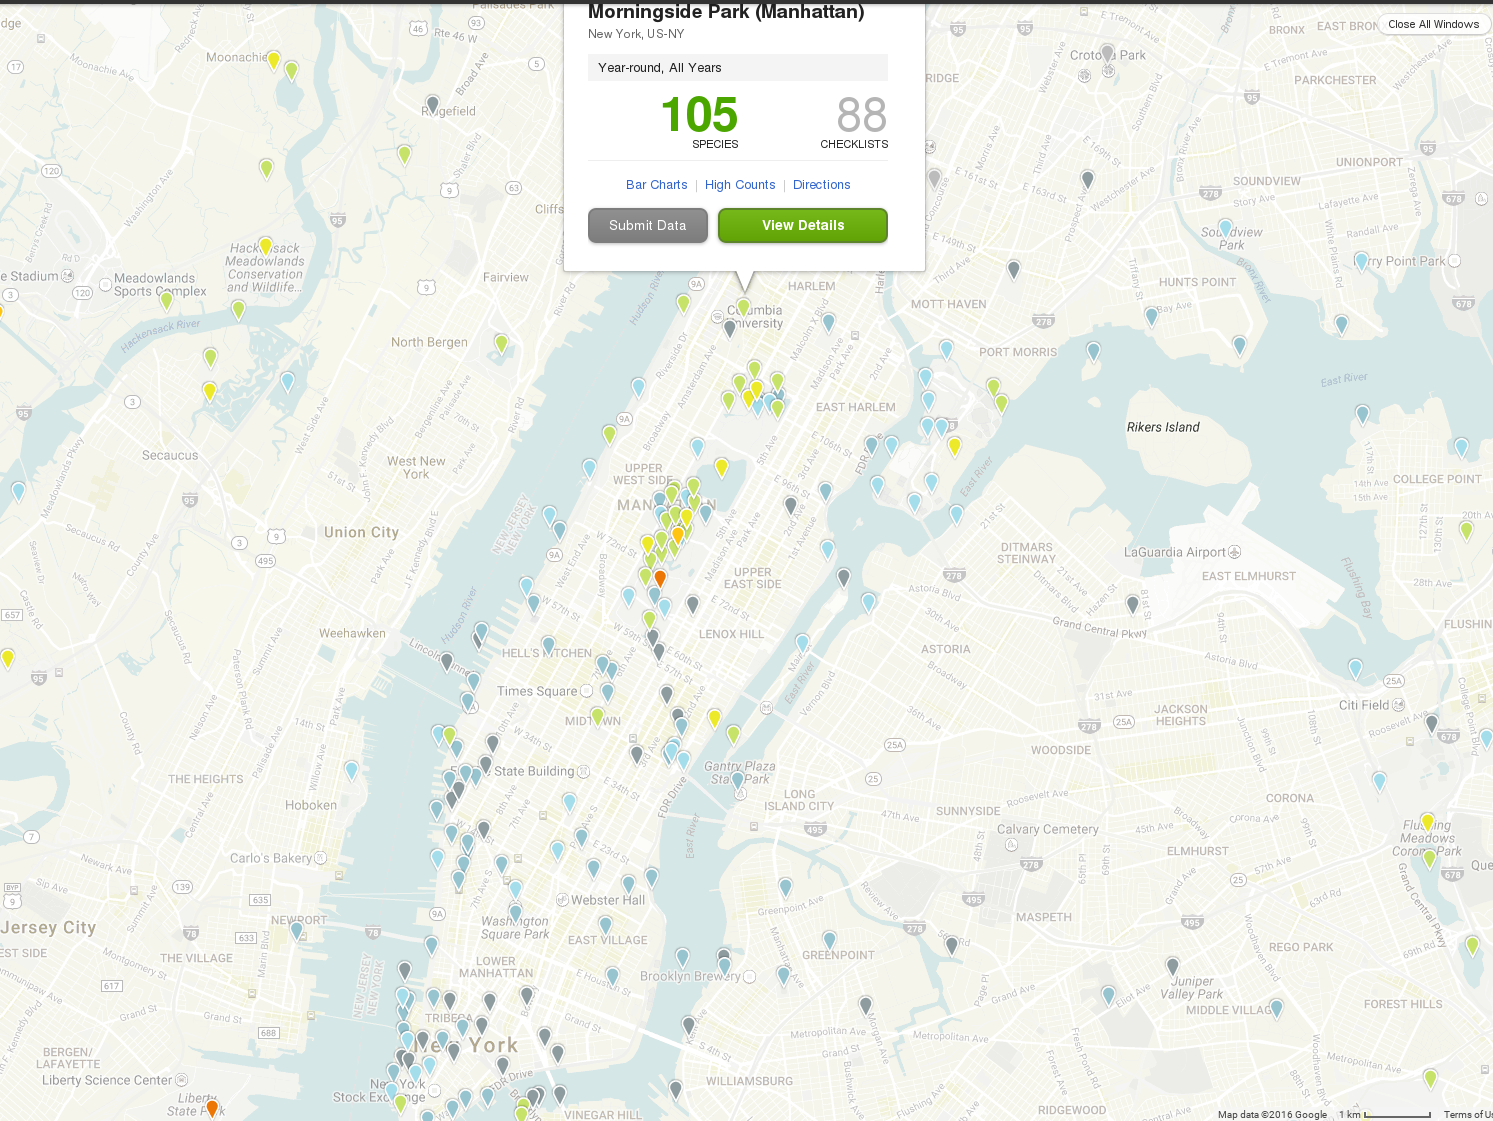
\includegraphics[width=0.8\textwidth]{ebird-checklist-manhattan.png}
    \caption{eBird checklist submissions on Manhattan island. (I believe) Checklists are aggregated by a number of sites for better plot. The location at CU is mistakenly labeled as Morningside Park. Zoom in for better view. }
    \label{fig1}
\end{figure}


Each checklist contains its location (latitude \& longitude), time point, and a list of bird counts for 953 species. Two sets of covariates are associated to each checklist. The first set ($\approx$ 12) of covariates describe the environmental information, such as elevation, temperature, and vegetation coverage, and explain why the bird is there. The second set ($\approx$4) of covariates are about the observation process and states how the observation is made, such as the type of observation (staitionary, traveling, area survey, etc.) and duration of observation. 

There are about 6 million checklists during the last 5 years (from 2010 to 2014). 

In this work, we would like to discover bird relations by bird embedding. The idea of bird embedding originates from word embedding in NLP, where various relations among words are discovered[citation of word embedding]. In this work, we would like to discover relations among birds by applying the embedding technique to the eBird data. 

Dispite its similarity with word embedding, there are new problems to consider for bird embedding. 
\begin{itemize}
\item Large quantity of data, which has 6 millions observations.
\item Rich information about checklists. In another word, checklists are not from the same distribution. We should construct a model in which environmental covariates expain presence/absence of species, and bird embedding captures interactions among species.  
\item Locations near each other should have similar distribution of birds, not only because they share similar covariates, but also because birds fly around. How to smooth the distribution?
\item How can we explain the embedding result? Making recommendation may not be a good idea here. 
\end{itemize}


\section{Bird Embedding}

The first model to consider is the combination of exponential family embedding and the exposure model.

In the embedding model, we essentially need to define the conditional distribution of the bird count of a species in a checklist given its {\it context}. Since we are interested in relationships among bird species, the {\it context} of a bird count is the vector of bird counts of other species in the checklist. Due to the generality of context, we can define the context of a bird count flexibly, for example, as bird counts of other species averaged over checklists within some radius of the current observation. The average may give more stable results, but we will consider this later. 

The exposure model can be used to describe the observation process. Mathematically, it plays the role of down-weighting zero entries in the observation matrix. In another word, a species is not observed either because no such bird lives there or because it is not detected by that observation. If the model choose the second explanation, then model would use little strength to fit the zero value. We will see this after we have defined the model formally.  

Let's define the model. Suppose there are $M$ checklists, and let $i$, $1 \le i \le M$, index checklists. In the data there are $N = 953$ species, each of which is indexed by $j$, $1 \le j \le N$.  
In each checklist $i$, $y_{ij}$ birds are observed for species $j$. The context of $y_{ij}$ is $\mathbf{c}_{ij} = (y_{i1}, \ldots, y_{i(j-1)}, y_{i(j+1)}, \ldots, y_{iN})$. For each checklist, the feature vector $\mathbf{x}_{i}$ brings some information of the observation process. The probability $u_{ij}$ of observing each species $j$ is calculated as $u_{ij} = \mathrm{logistic}(\beta_j^\top \mathbf{x}_i)$, where $\beta_j$ is a parameter. The indicator $a_{ij}$ of observing species $j$ at checklist $i$ is sampled from Bernoulli distribution. 
\begin{eqnarray}
a_{ij} &\sim& \mathrm{Bernoulli}(u_{ij}).
\end{eqnarray}

The observed count $y_{ij}$ is from Poisson distribution defined as follows.   
\begin{eqnarray}
y_{ij} &\sim& \mathrm{Poisson}(a_{ij} \lambda_{ij}),
\end{eqnarray}
where 
\begin{eqnarray}
\lambda_{ij} = \exp(\theta_{j}^\top \mathbf{c}_{ij} ),
\end{eqnarray}
where the vector $\theta_j$ is a parameter shared by species $j$. 

The parameter $\theta_j$ and $\beta_j$ are given Gaussian priors. 
\begin{eqnarray}
\theta_j &\sim& \mathrm{Normal}(\mathbf{0}, \sigma_1 I), \\
\beta_j &\sim& \mathrm{Normal}(\mathbf{0}, \sigma_2 I),
\end{eqnarray}
where $\sigma_1$ and $\sigma_2$ are hyper-parameters, $\mathbf{0}$ is a zero vector with length $N$, and $I$ is the identity matrix of size $N$. 


The definition above is made for all $1 \le i \le M$ and $1 \le j \le N$. 

What is the indication of the learned parameter $\theta$? It is easy to see that $\theta$ captures the correlation among bird species. For example, if we see a {\it sea gull}, which is a strong indication of the location being at the coast, which in turns has positive indication of {\it albatross}. In this sense, the correlation among bird species does not necessarily indicates interactions among them. Instead, their distributions are caused by some common hidden factors and correlated when these hidden factors are marginalized (or excluded from the model). As a second step, we should include environmental covariates and let them explain distributions of birds. We can define the Poisson rate $\lambda$ as follows. 
\begin{eqnarray}
\lambda_{ij} =  \exp(\theta_{j}^\top \mathbf{c}_{ij} ) + f_j (\mathbf{v}_i)
\end{eqnarray}
where $f_i$ is a function that maps the covariates $\mathbf{v}_i$ at location $i$ to a fitness value for species $j$. If $f_j (\mathbf{v}_i)$ can perfectly model species distributions for single species, then $\theta$ will capture interactions among species. However, it is more likely that there are still some factors not included in $\mathbf{v}$. Nevertheless, $\theta$ will contain both the marginalized correlation and interactions among birds. Experts may be able to identify factors missing from $\mathbf{v}$ or manually discover more bird interactions from $\theta$.  

The function $f_j (\mathbf{v}_i)$ should be learned first, so the species distribution is explained by environmental covariates first. The embedding model is used to explain the part not explained by $f$. Compared with joint learning of $f$ and $\theta$, there are two benefits from this considerations: a) the embedding part can focus more on interactions among bird species, and b) learning is computationally more efficient. 

\section{Research Directions}

Assumption: embeddings at similar time-locations are similar but different. Can we use a $\theta_{ij}$ for each checklist $i$ and species $j$ and put a GP prior over $\theta_{ij}$-s to encourage strong correlation among $\theta_{ij}$-s at neighboring locations?  

Can we do inference over 6 million checklists?

Can we predict the presence/absence of species?

\section{TODO list}
\begin{itemize}
\item Derivation of the inference method
\item Run a small dataset with the P-EMB model
\item ...
\end{itemize}


\end{document}
